\documentclass[11pt,letterpaper]{article}\usepackage[]{graphicx}\usepackage[]{color}
% maxwidth is the original width if it is less than linewidth
% otherwise use linewidth (to make sure the graphics do not exceed the margin)
\makeatletter
\def\maxwidth{ %
  \ifdim\Gin@nat@width>\linewidth
    \linewidth
  \else
    \Gin@nat@width
  \fi
}
\makeatother

\definecolor{fgcolor}{rgb}{0.345, 0.345, 0.345}
\newcommand{\hlnum}[1]{\textcolor[rgb]{0.686,0.059,0.569}{#1}}%
\newcommand{\hlstr}[1]{\textcolor[rgb]{0.192,0.494,0.8}{#1}}%
\newcommand{\hlcom}[1]{\textcolor[rgb]{0.678,0.584,0.686}{\textit{#1}}}%
\newcommand{\hlopt}[1]{\textcolor[rgb]{0,0,0}{#1}}%
\newcommand{\hlstd}[1]{\textcolor[rgb]{0.345,0.345,0.345}{#1}}%
\newcommand{\hlkwa}[1]{\textcolor[rgb]{0.161,0.373,0.58}{\textbf{#1}}}%
\newcommand{\hlkwb}[1]{\textcolor[rgb]{0.69,0.353,0.396}{#1}}%
\newcommand{\hlkwc}[1]{\textcolor[rgb]{0.333,0.667,0.333}{#1}}%
\newcommand{\hlkwd}[1]{\textcolor[rgb]{0.737,0.353,0.396}{\textbf{#1}}}%
\let\hlipl\hlkwb

\usepackage{framed}
\makeatletter
\newenvironment{kframe}{%
 \def\at@end@of@kframe{}%
 \ifinner\ifhmode%
  \def\at@end@of@kframe{\end{minipage}}%
  \begin{minipage}{\columnwidth}%
 \fi\fi%
 \def\FrameCommand##1{\hskip\@totalleftmargin \hskip-\fboxsep
 \colorbox{shadecolor}{##1}\hskip-\fboxsep
     % There is no \\@totalrightmargin, so:
     \hskip-\linewidth \hskip-\@totalleftmargin \hskip\columnwidth}%
 \MakeFramed {\advance\hsize-\width
   \@totalleftmargin\z@ \linewidth\hsize
   \@setminipage}}%
 {\par\unskip\endMakeFramed%
 \at@end@of@kframe}
\makeatother

\definecolor{shadecolor}{rgb}{.97, .97, .97}
\definecolor{messagecolor}{rgb}{0, 0, 0}
\definecolor{warningcolor}{rgb}{1, 0, 1}
\definecolor{errorcolor}{rgb}{1, 0, 0}
\newenvironment{knitrout}{}{} % an empty environment to be redefined in TeX

\usepackage{alltt} 
\usepackage[utf8]{inputenc} 
\usepackage[spanish, es-tabla, es-nodecimaldot]{babel} % Formato a español
\usepackage[T1]{fontenc}    % Permite utilizar otras tipografías
\usepackage[vmargin=2.5cm,hmargin=2cm]{geometry}
\usepackage{multicol}   % Unir columnas en tablas y formato a dos columnas
\usepackage{multirow}   % Unir filas en tablas
\usepackage{graphicx}   % Necesario para insertar gráficas
\usepackage{float}      % Corregir ubicación de imágenes y tablas
%\usepackage{subfigure} % Insertar subfiguras
%\usepackage{url}       % Hiervínculo a direcciones URL
\usepackage{listings}
\usepackage{flushend}
\usepackage{minted}
\usepackage[none]{hyphenat} % Permite utilizar el comando \sloppy
\usepackage[small]{caption}	% Reduce el tamaño de letra utilizado en los pies de figura.
\usepackage{hyperref}   % Agrega enlaces internos de las secciones, figuras y tablas.
\usepackage{color}      % Definición de colores
    \hypersetup{colorlinks=true, linkcolor=[rgb]{0,0,1}, citecolor=[rgb]{0,0,1}}
\usepackage{xcolor}		% Permite definir un color para utilizarlo dentro del documento.
    \definecolor{gris}{RGB}{70,70,70}	% Definiendo el color gris
    \definecolor{negro}{RGB}{40,40,40}		% Definiendo el color negro

%%%%%%%% Modificación de los espacios de los títulos de secciones %%%%%%%%%%
\usepackage{titlesec}		% Permite reconfigurar  los títulos de las secciones y subsecciones
\renewcommand\thesection{\Roman{section}}	% Numeración romana en las secciones
\renewcommand\thesubsection{\Roman{subsection}}		% Numeración romana en las subsecciones
\titlespacing*{\section}{0pt}{2.5mm}{0mm}	% Espaciado del título {espacio izquierdo}{arriba del título}{abajo del título}
\titleformat{\section}[block]{\large\scshape\centering}{\thesection.}{1em}{}	% Espaciado del título de las secciones
\titleformat{\subsection}[block]{\large}{\thesubsection.}{1em}{}				% Espaciado del título de las subsecciones
%%%%%%%%%%%%%%%%%%%%%%%%%%%%%%%%%%%%%%%%%%%%%%%%%%%%%%%%%%%%%%%%%%%%%%%%%%%%%%

%Se define un comando \colorhrule para hacer líneas horizontales de color con 3 argumentos: color, largo, ancho.
\newcommand{\colorhrule}[3]{\begingroup\color{#1}\rule{#2}{#3}\endgroup}

\setlength{\intextsep}{1mm} % Distancia superior e inferior en objetos flotantes
\setlength{\columnsep}{5mm} % Separación entre columnas del documento
\IfFileExists{upquote.sty}{\usepackage{upquote}}{}
\begin{document}
\sloppy     % Evita que las palabras se corten al saltar de línea.
\begin{center}
\begin{tabular}{cc}
\multirow{2}{3.5cm}{
\includegraphics[width=4cm]{UEBlogo.png}}	& \huge{\textsc{\textbf{Universidad El Bosque}}}\\ %\vspace{5mm}
 & \scriptsize{\textsc{FACULTAD DE CIENCIAS}}\\[5mm]
 & \Large{\textsf{\textbf{Modelos ML para regresión y clasificación}}}\\
 & \small{\textsf{Angie Caterine Sarmiento Gonzalez [1233507154]}}\\ \vspace{5mm}
 %& \small{\textsf{Nombre completo de alumno 2 [Código]}}\\
 & \small{\textsc{Estadística $|$ Minería de Datos}}\\
 & \today\\
\end{tabular}
\end{center}
\begin{center}
\colorhrule{black}{16.5cm}{1.2pt}
\end{center}

\section*{\textbf{Actividad}}

Construir y validar el modelo de regresión más potente para predecir el precio de venta Price de un automóvil nuevo con base en las variables predictoras $X1$=KM (kilometraje), $X2$=Age (años de uso) y $X3$=Weight (peso)

\section*{\textbf{Pasos a seguir}}
\begin{enumerate}
    \item Seleccione en un mismo data frame las variables de interés.


\begin{knitrout}
\definecolor{shadecolor}{rgb}{0.969, 0.969, 0.969}\color{fgcolor}\begin{kframe}
\begin{verbatim}
## # A tibble: 6 x 4
##      KM   Age Weight Price
##   <dbl> <dbl>  <dbl> <dbl>
## 1 46986    23   1165 13500
## 2 72937    23   1165 13750
## 3 41711    24   1165 13950
## 4 48000    26   1165 14950
## 5 38500    30   1170 13750
## 6 61000    32   1170 12950
\end{verbatim}
\end{kframe}
\end{knitrout}

\texttbf{Exploración de los datos}
\\ \\
Se realiza una visualización de la distribución de la variable de respuesta para encontrar el modelo más optimo que prediga los datos.
\begin{knitrout}
\definecolor{shadecolor}{rgb}{0.969, 0.969, 0.969}\color{fgcolor}
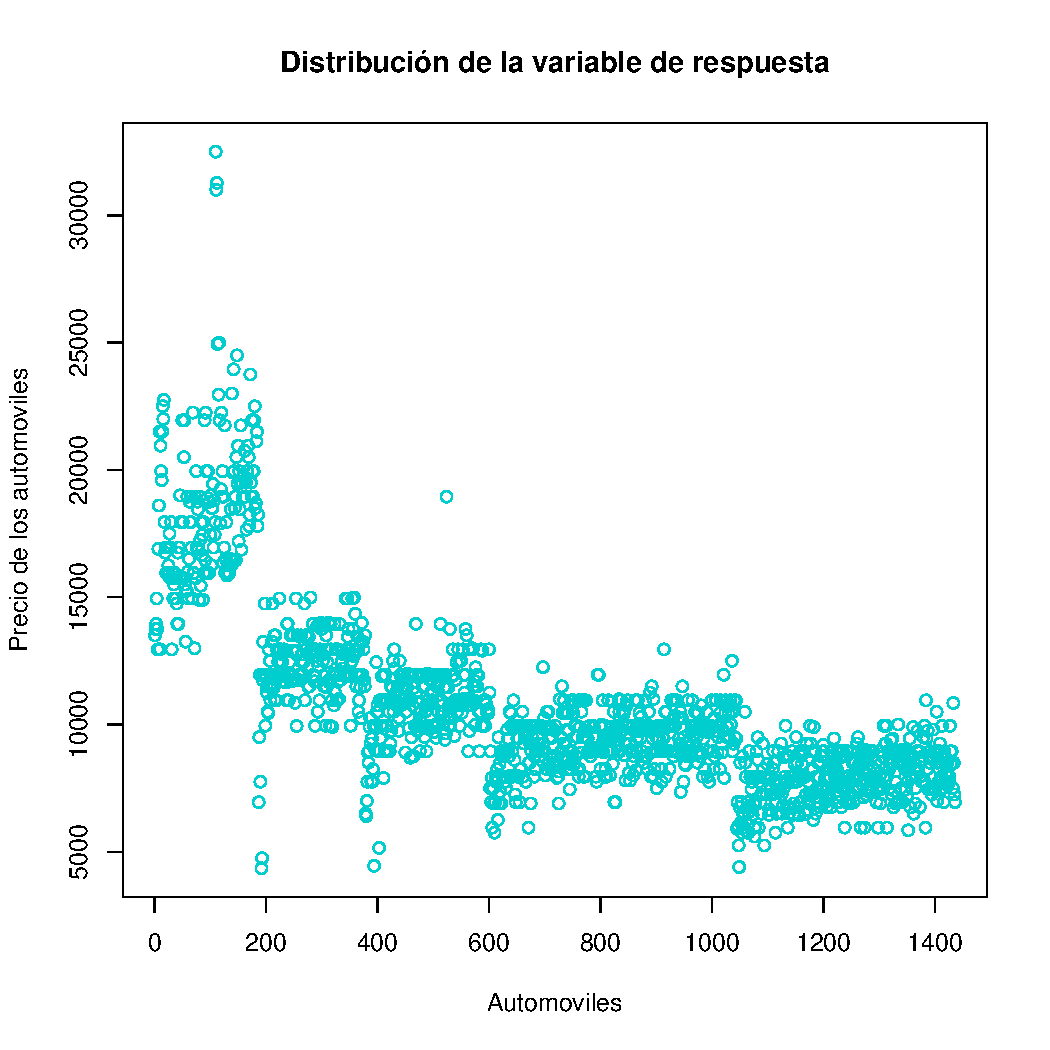
\includegraphics[width=\maxwidth]{figure/unnamed-chunk-3-1} 

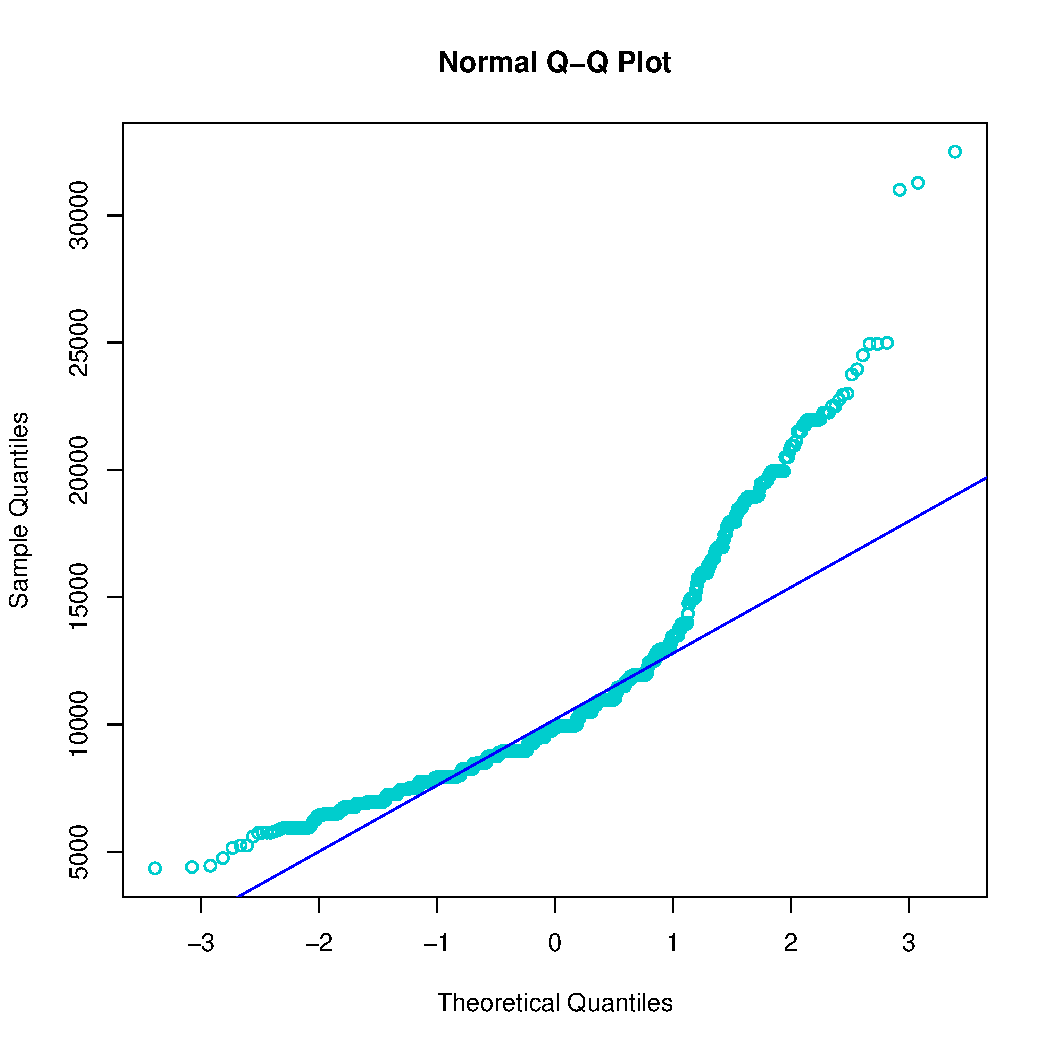
\includegraphics[width=\maxwidth]{figure/unnamed-chunk-3-2} 

\end{knitrout}
Parece ser que hay evidencia para rechazar normalidad de la varible precio. 
\\\\
\texttbf{Distribución del precio de los datos explicado por cada una de las variables}
\begin{knitrout}
\definecolor{shadecolor}{rgb}{0.969, 0.969, 0.969}\color{fgcolor}
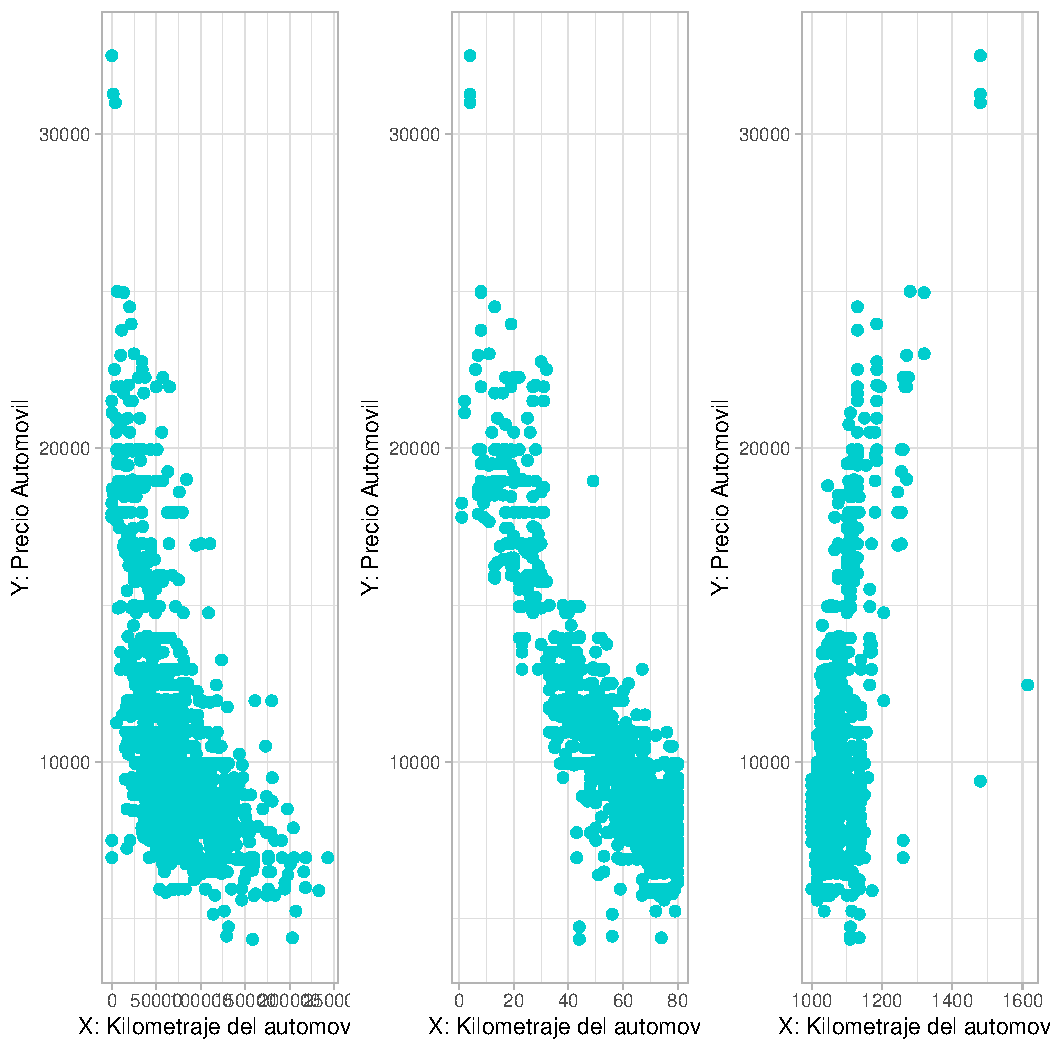
\includegraphics[width=\maxwidth]{figure/unnamed-chunk-4-1} 

\end{knitrout}

Hay una tendencia de disminución de precio al comparar precio del auto con  las variables Age y kM

    \item Construya una conjunto de entrenamiento (75\%) y otro de prueba (25\%). Tome la semilla 12345
\begin{knitrout}
\definecolor{shadecolor}{rgb}{0.969, 0.969, 0.969}\color{fgcolor}\begin{kframe}
\begin{alltt}
\hlcom{# Seleccionar siempre la misma partición}
\hlkwd{set.seed}\hlstd{(}\hlnum{12345}\hlstd{)}

\hlcom{# Muestra aleatoria del 75% de las filas del }
\hlcom{#conjunto "datos" para el conjunto de entrenamiento}

\hlstd{train.filas}\hlkwb{<-}\hlkwd{sample}\hlstd{(}\hlkwc{x}\hlstd{=}\hlkwd{row.names}\hlstd{(datos),}\hlkwc{size} \hlstd{=} \hlkwd{dim}\hlstd{(datos)[}\hlnum{1}\hlstd{]}\hlopt{*}\hlnum{0.75}\hlstd{)}

\hlcom{# CONJUNTO DE ENTRENAMIENTO (selección de columnas)}
\hlstd{train.set}\hlkwb{<-}\hlstd{datos[train.filas,]}
\hlstd{train1}\hlkwb{<-}\hlstd{train.set} \hlopt \hlkwd{mutate_if}\hlstd{(is.numeric,scale)}
\hlkwd{dim}\hlstd{(train.set)}
\end{alltt}
\begin{verbatim}
## [1] 1077    4
\end{verbatim}
\begin{alltt}
\hlcom{# CONJUNTO DE PRUEBA}
\hlstd{test.filas}\hlkwb{<-}\hlkwd{setdiff}\hlstd{(}\hlkwc{x} \hlstd{=} \hlkwd{row.names}\hlstd{(datos),train.filas)}
\hlstd{test.set}\hlkwb{<-}\hlstd{datos[test.filas,]}
\hlstd{test.set1}\hlkwb{<-} \hlstd{test.set} \hlopt \hlkwd{mutate_if}\hlstd{(is.numeric,scale)}
\hlkwd{dim}\hlstd{(test.set)}
\end{alltt}
\begin{verbatim}
## [1] 359   4
\end{verbatim}
\end{kframe}
\end{knitrout}

    \item Entrene los cinco modelos con base en el conjunto de entrenamiento y almacene los correspondientes precios predichos para los automóviles de dicho conjunto.
    \\ \\
    \textbf{Modelo 1}: un modelo de regresión lineal múltiple:
    \[Y= \beta_0 + \beta_1X_1 + \beta_2X_2 + \beta_3X_3 + \epsilon\]
\begin{knitrout}
\definecolor{shadecolor}{rgb}{0.969, 0.969, 0.969}\color{fgcolor}\begin{kframe}
\begin{alltt}
\hlstd{modelo1}\hlkwb{<-}\hlkwd{lm}\hlstd{(Price}\hlopt{~}\hlstd{KM}\hlopt{+}\hlstd{Age}\hlopt{+}\hlstd{Weight,}\hlkwc{data}\hlstd{=train.set)}
\end{alltt}
\end{kframe}
\end{knitrout}
\[\widehat{Price}= -3189.31 -0.02 \cdot KM-117.76 \cdot Age + 20.71 \cdot Weight\]
    \textbf{Modelo 2}:un modelo de regresión múltiple de grado 3:
    \[Y= \beta_0 + \beta_1X_1 + \beta_2X_2^2 + \beta_3X_3^3 + \epsilon\]
\begin{knitrout}
\definecolor{shadecolor}{rgb}{0.969, 0.969, 0.969}\color{fgcolor}\begin{kframe}
\begin{alltt}
\hlstd{modelo2}\hlkwb{<-}\hlkwd{lm}\hlstd{(Price}\hlopt{~}\hlstd{KM}\hlopt{+}\hlstd{(Age}\hlopt{^}\hlnum{2}\hlstd{)}\hlopt{+}\hlstd{(Weight}\hlopt{^}\hlnum{3}\hlstd{),}\hlkwc{data}\hlstd{=train.set)}
\end{alltt}
\end{kframe}
\end{knitrout}
\[\widehat{Price}= -3189.31 -0.02 \cdot KM-117.76 \cdot Age^2 + 20.71 \cdot Weight^3\]

    \textbf{Modelo 3}:Un modelo ajustado por algoritmo kNN con $k=10$ vecinos más próximos.
    
\begin{knitrout}
\definecolor{shadecolor}{rgb}{0.969, 0.969, 0.969}\color{fgcolor}\begin{kframe}
\begin{alltt}
\hlstd{modelo3}\hlkwb{<-}\hlstd{FNN}\hlopt{::}\hlkwd{knn.reg}\hlstd{(}\hlkwc{train} \hlstd{= train.set,}\hlkwc{y} \hlstd{=train.set}\hlopt{$}\hlstd{Price,}\hlkwc{k} \hlstd{=} \hlnum{10}\hlstd{)}
\end{alltt}
\end{kframe}
\end{knitrout}
     \textbf{Modelo 4}:Un modelo ajustado por algoritmo kNN con $k=10$ vecinos más próximos sobre las variables normalizadas $Z_1$, $Z_2$ y $Z_3$.
\begin{knitrout}
\definecolor{shadecolor}{rgb}{0.969, 0.969, 0.969}\color{fgcolor}\begin{kframe}
\begin{alltt}
\hlstd{modelo4}\hlkwb{<-}\hlstd{FNN}\hlopt{::}\hlkwd{knn.reg}\hlstd{(}\hlkwc{train} \hlstd{=train1 ,}\hlkwc{y} \hlstd{=train1}\hlopt{$}\hlstd{Price,}\hlkwc{k} \hlstd{=} \hlnum{10}\hlstd{)}
\end{alltt}
\end{kframe}
\end{knitrout}

     \textbf{Modelo 5}: Un modelo loglineal
\begin{knitrout}
\definecolor{shadecolor}{rgb}{0.969, 0.969, 0.969}\color{fgcolor}\begin{kframe}
\begin{alltt}
\hlstd{modelo5} \hlkwb{=} \hlkwd{lm}\hlstd{(Price}\hlopt{~}\hlstd{KM}\hlopt{+}\hlstd{Age}\hlopt{+}\hlstd{Weight,}\hlkwc{data}\hlstd{=train.set)}
\end{alltt}
\end{kframe}
\end{knitrout}

     
\begin{knitrout}
\definecolor{shadecolor}{rgb}{0.969, 0.969, 0.969}\color{fgcolor}\begin{kframe}
\begin{verbatim}
## # A tibble: 1,077 x 9
##        KM   Age Weight Price Price_pred1 Price_pred2 Price_pred3 Price_pred4
##     <dbl> <dbl>  <dbl> <dbl>       <dbl>       <dbl>       <dbl>       <dbl>
##  1  21684    19   1185 23950      18581.      18581.      20584        3.00 
##  2  62636    22   1255 17950      18680.      18680.      15575        2.28 
##  3  88807    68   1050  8500       8382.       8382.       8505       -0.646
##  4  86714    68   1035  8950       8122.       8122.       8525       -0.582
##  5  81930    76   1070  7750       8021.       8021.       7844.      -0.825
##  6 110287    68   1050  9500       7859.       7859.       9115       -0.330
##  7  69103    68   1035  9750       8551.       8551.       9530       -0.236
##  8 204250    68   1115  7900       6917.       6917.       6305       -1.14 
##  9  29650    55   1025  9950      10835.      10835.      10170       -0.170
## 10  57000    80   1000  7750       6708.       6708.       8255       -0.793
## # ... with 1,067 more rows, and 1 more variable: Price_pred5 <dbl>
\end{verbatim}
\end{kframe}
\end{knitrout}



    \item Estime (y almacene) los correspondientes errores cuadráticos medios de entrenamiento MSEE de los cinco modelos ¿Cuál modelo ajustó mejor al conjunto de entrenamiento?
\begin{knitrout}
\definecolor{shadecolor}{rgb}{0.969, 0.969, 0.969}\color{fgcolor}\begin{kframe}
\begin{verbatim}
##    MSE_m3  MSE_m1  MSE_m2  MSE_m5    MSE_m4
## 1 1118598 1957205 1957205 1957205 129063302
\end{verbatim}
\end{kframe}
\end{knitrout}
   
   El modelo que mejor se ajusto fue el modelo no párametrico KNN con k=10, ya que su error cuadratico medio es el mas bajo.\\
    \item Evalúe los modelos entrenados en el paso 4 utilizando el conjunto de prueba y almacene los correspondientes precios predichos para los automóviles de dicho conjunto.
\begin{knitrout}
\definecolor{shadecolor}{rgb}{0.969, 0.969, 0.969}\color{fgcolor}\begin{kframe}
\begin{verbatim}
## # A tibble: 359 x 9
##       KM   Age Weight Price Price_pred1 Price_pred2 Price_pred3 Price_pred4
##    <dbl> <dbl>  <dbl> <dbl>       <dbl>       <dbl>       <dbl>       <dbl>
##  1 72937    23   1165 13750      16448.      16448.      12135        0.825
##  2 41711    24   1165 13950      17091.      17091.      14147        1.08 
##  3 75889    30   1245 18600      17209.      17209.      14225        2.15 
##  4 31461    25   1185 20950      17637.      17637.      19895        2.70 
##  5 18739    28   1185 22000      17593.      17593.      20475        2.82 
##  6 34000    30   1185 22750      16986.      16986.      20025        2.92 
##  7 64359    30   1105 16950      14591.      14591.      15725        1.43 
##  8 43905    29   1170 16950      16552.      16552.      15846.       1.88 
##  9 56349    28   1120 15950      15332.      15332.      14010        1.45 
## 10 41000    22   1100 15500      15998.      15998.      14774.       1.42 
## # ... with 349 more rows, and 1 more variable: Price_pred5 <dbl>
\end{verbatim}
\end{kframe}
\end{knitrout}
    \item Estime (y almacene) los correspondientes errores cuadráticos medios de prueba MSEP de los cinco modelos.
\begin{knitrout}
\definecolor{shadecolor}{rgb}{0.969, 0.969, 0.969}\color{fgcolor}\begin{kframe}
\begin{verbatim}
##    MSEP_m3 MSEP_m1 MSEP_m2 MSEP_m5   MSEP_m4
## 1 867725.3 2130161 2130161 2130161 125969090
\end{verbatim}
\end{kframe}
\end{knitrout}
    
    \item Compare visualmente los MSEE y MSEP de los cinco modelos. A su criterio ¿Cuál modelo escogería para predecir el precio de nuevos autos? Justifique
\begin{knitrout}
\definecolor{shadecolor}{rgb}{0.969, 0.969, 0.969}\color{fgcolor}
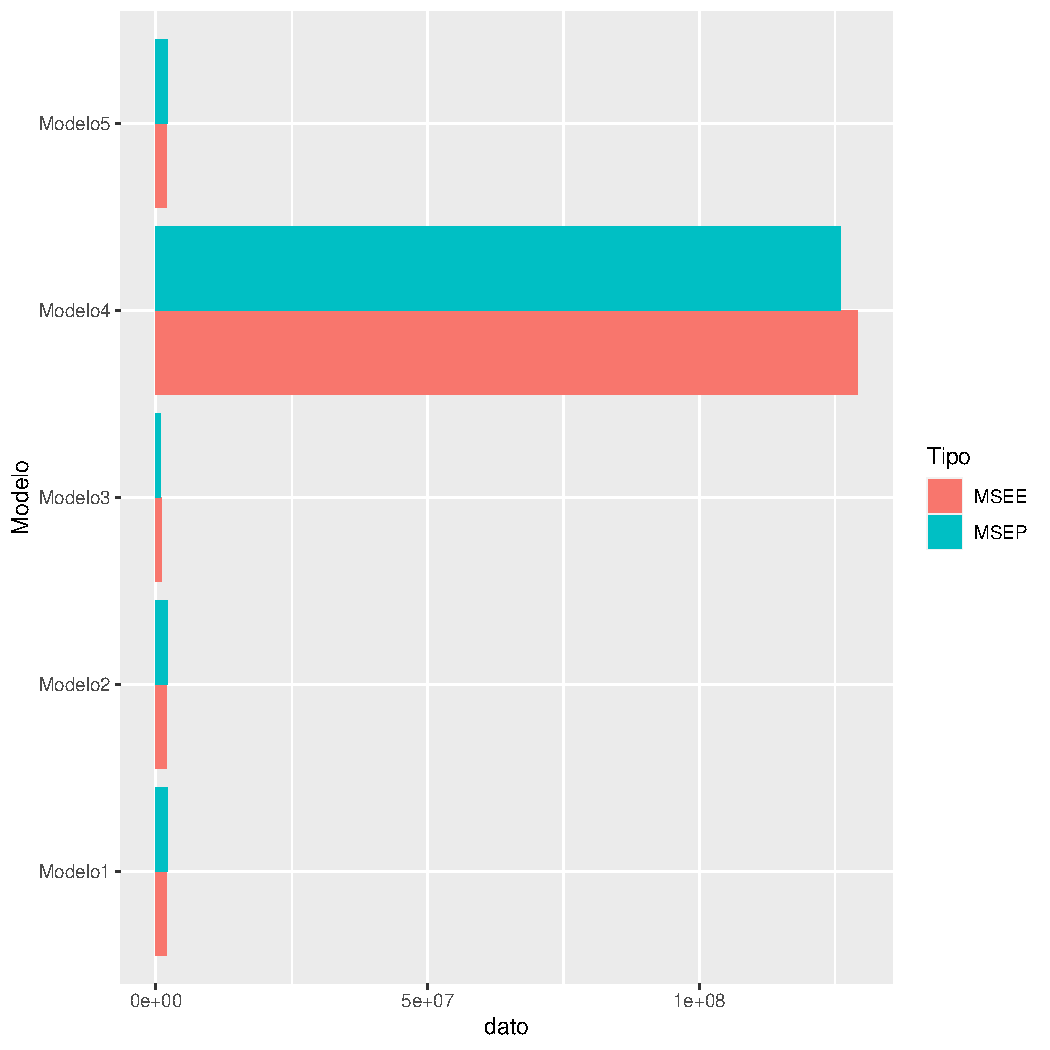
\includegraphics[width=\maxwidth]{figure/unnamed-chunk-15-1} 
\begin{kframe}\begin{verbatim}
##           dato  Modelo Tipo
## 1    1957204.9 Modelo1 MSEE
## 2    1957204.9 Modelo2 MSEE
## 3    1118598.3 Modelo3 MSEE
## 4  129063302.1 Modelo4 MSEE
## 5    1957204.9 Modelo5 MSEE
## 6    2130161.4 Modelo1 MSEP
## 7    2130161.4 Modelo2 MSEP
## 8     867725.3 Modelo3 MSEP
## 9  125969090.3 Modelo4 MSEP
## 10   2130161.4 Modelo5 MSEP
\end{verbatim}
\end{kframe}
\end{knitrout}
 
\begin{knitrout}
\definecolor{shadecolor}{rgb}{0.969, 0.969, 0.969}\color{fgcolor}\begin{kframe}
\begin{verbatim}
##       dato  Modelo Tipo
## 1 867725.3 Modelo3 MSEP
\end{verbatim}
\end{kframe}
\end{knitrout}
  
  Se escoge el modelo 3 ya que tiene el menor MSEE 
    \item Con base en el modelo que seleccionó en el punto 7, prediga el precio que tendrán los siguientes tres automóviles con perfiles:
    \begin{table}[H]
        \centering
        \begin{tabular}{|c|c|c|c|}\hline
           \textbf{Automovil}  &  \textbf{KM} & \textbf{Age} & \textbf{Weight} \\ \hline
             1 & 60.000 &30 & 1.300 \\ \hline
            2 & 22.000 & 25  & 1.500 \\ \hline
           3 &  3.000 & 4  & 1.070 \\ \hline
            
        \end{tabular}
        \caption{Caracteristicas de los nuevos autos}
        \label{tab:my_label}
    \end{table}
    
Estimación de precios para los nuevos autos mediante el modelo KNN con k=10
\begin{knitrout}
\definecolor{shadecolor}{rgb}{0.969, 0.969, 0.969}\color{fgcolor}\begin{kframe}
\begin{alltt}
\hlstd{nuevo}\hlkwb{<-} \hlkwd{tibble}\hlstd{(}\hlkwc{KM}\hlstd{=}\hlkwd{c}\hlstd{(}\hlnum{60.000}\hlstd{,}\hlnum{22.000}\hlstd{,}\hlnum{3.000}\hlstd{),}\hlkwc{Age}\hlstd{=}\hlkwd{c}\hlstd{(}\hlnum{30}\hlstd{,}\hlnum{25}\hlstd{,}\hlnum{4}\hlstd{),}\hlkwc{Weight}\hlstd{=}\hlkwd{c}\hlstd{(}\hlnum{1.300}\hlstd{,}\hlnum{1.500}\hlstd{,}\hlnum{1.070}\hlstd{))}

\hlkwd{knn.reg}\hlstd{(}\hlkwc{train} \hlstd{= train.set[}\hlopt{-}\hlnum{4}\hlstd{],} \hlcom{# Sólo predictoras de train.set}
        \hlkwc{test} \hlstd{= nuevo,}   \hlcom{# Sólo predictoras de test.set}
        \hlkwc{y} \hlstd{= train.set}\hlopt{$}\hlstd{Price,}   \hlcom{# Sólo respuesta de train.set}
        \hlkwc{k} \hlstd{=} \hlnum{10}\hlstd{)}
\end{alltt}
\begin{verbatim}
## Prediction:
## [1] 17738.5 17738.5 17738.5
\end{verbatim}
\end{kframe}
\end{knitrout}
 
 \begin{table}[H]
        \centering
        \begin{tabular}{|c|c|c|c|c|}\hline
           \textbf{Automovil}  &  \textbf{KM} & \textbf{Age} & \textbf{Weight} & Precio Estimado \\ \hline
             1 & 60.000 &30 & 1.300 & 17738.5 \\ \hline
            2 & 22.000 & 25  & 1.500 & 17738.5 \\ \hline
           3 &  3.000 & 4  & 1.070  & 17738.5\\ \hline
            
        \end{tabular}
        \caption{Predicción del precio de los nuevos autos}
        

        \label{tab:my_label}
    \end{table}
\end{enumerate}
\begin{thebibliography}{1} % Bibliography - this is intentionally simple in this template
\bibitem{presentation} Ramos David,
\newblock{\em Evaluación de modelos para regresión: Ejemplo},
\newblock  (2020).

\end{thebibliography}
\end{document}
